% Chapter 1

\chapter{Introducción general} % Main chapter title

\label{Chapter1} % For referencing the chapter elsewhere, use \ref{Chapter1} 
\label{IntroGeneral}

%----------------------------------------------------------------------------------------

% Define some commands to keep the formatting separated from the content 
\newcommand{\keyword}[1]{\textbf{#1}}
\newcommand{\tabhead}[1]{\textbf{#1}}
\newcommand{\code}[1]{\texttt{#1}}
\newcommand{\file}[1]{\texttt{\bfseries#1}}
\newcommand{\option}[1]{\texttt{\itshape#1}}
\newcommand{\grados}{$^{\circ}$}

%----------------------------------------------------------------------------------------

%\section{Introducción}

En esta sección se da una explicación general de los temas sobre los cuales se basa este trabajo. Se dará una introducción al protocolo CAN - \textit{Controller Area Network} y a qué es un servomotor. También se hablará sobre el proyecto SN-17 y la motivación y alcance del trabajo, así como el estado del arte de esta tecnología.

%----------------------------------------------------------------------------------------
\section{Controller Area Network - CAN}

\textit{Controller Area Network} o CAN es un protocolo de comunicación desarrollado por Bosch \citep{wikipedia_CAN} orientado originalmente a la industria automotriz, y hoy en día es empleado en muchas otras aplicaciones. En el año 1991 Bosch publicó la especificación CAN 2.0 donde se diferencian aspectos de identificación de dispositivos conectados en la red y, en el año 1993, se estandarizó el protocolo bajo la norma internacional ISO 11898 \citep{web_ISO_CAN}.

CAN se caracteriza por su robustez y bajos requerimientos de cableado. En su concepción, se pensó para proveer comunicaciones deterministicas en sistemas complejos, teniendo las siguientes cualidades \citep{Understanding_CAN}:
\begin{itemize}
	\item Prioridad de mensajes y latencia máxima asegurada.
	\item Comunicaciones a varios dispositivos al mismo tiempo.	
	\item Bus multi-maestro.
	\item Detección de errores en nodos y mensajes.
	\item Protocolo asincrónico - sin línea de clock.
\end{itemize}

Para realizar la transferencia de información CAN emplea líneas de transmisión, comunmente llamados CAN High y CAN Low, y estos son los únicos enlaces requeridos. Al comienzo de cada mensaje, se emplea un identificador, que indica la prioridad del mensaje, así como a quien está dirigido. Usando esta información cada nodo de la red determina que hacer. En la Figura \ref{fig:canBus}, se puede ver un esquema básico de una red CAN.


\begin{figure}[htbp]
	\centering
	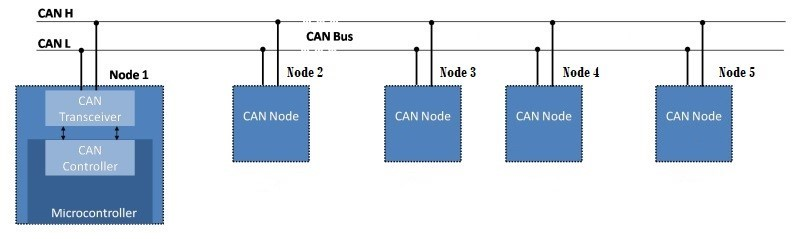
\includegraphics[scale=.6]{./Figures/CANBUS-Esquema.jpg}
	\caption{Esquema de red CAN\protect\footnotemark}
	\label{fig:canBus}
\end{figure}

\footnotetext{\url{https://www.seeedstudio.com/blog/2019/11/27/introduction-to-can-bus-and-how-to-use-it-with-arduino/}} %Link a imagen de Red CAN
%----------------------------------------------------------------------------------------

\section{Servomotores}

Un servomotor\citep{Industrial_Automation_Hands_On} es un tipo de motor eléctrico que tiene la capacidad de controlar la posición angular del eje, así como la velocidad de rotación y el torque. En general, el tipo de motor eléctrico que se emplee no determina si es o no un servomotor, sino que cuente las cualidades de control mencionadas. Para lograr esto, suele emplearse un sistema de lazo cerrado que se retroalimenta con la información proporcionada por un sensor que mide la posición angular del eje, llamado encoder. Esto es procesado por un controlador, quien se encarga de proporcionar la corriente adecuada a las bobinas del motor para que este se mueva de la forma indicada. En la Figura \ref{fig:servomotor} se puede ver un servomotor con sus distintas partes.

\begin{figure}[htbp]
	\centering
	\includegraphics[scale=0.6]{./Figures/servomotor.jpg}
	\caption{Esquema un servomotor\protect\footnotemark}
	\label{fig:servomotor}
\end{figure}

\footnotetext{\url{https://www.logicbus.com.mx/blog/que-es-un-servo-motor/}} %Link a imagen de servomotor

%----------------------------------------------------------------------------------------

\section{Proyecto SN-17 - Servo Nema 17}

El proyecto SN-17 es un sistema desarrollado por la organización A3 Engineering que permite convertir motores eléctricos del tipo paso a paso o \textit{steppers} en servomotores. Este tipo de motores tienen, similar a un servomotor, la capacidad de controlar su posición y velocidad, pero con un lazo de control abierto. En caso de que haya perturbaciones al funcionamiento normal, el motor pierde el control de la posición y debe realizar una rutina de \textit{homing} para recuperarlo. Esto puede traer problemas en ciertas aplicaciones de precisión. Además, son incapaces de entregar torque constante a la salida, por el mismo motivo. El sistema SN-17 agrega un encoder y un controlador al motor, generando un lazo cerrado y logrando las funcionalidades de un servomotor. En la Figura \ref{fig:SN17} se puede observar una placa de control SN-17. Esta se coloca en la parte trasera de un motor paso a paso y se lo conecta directamente.

\begin{figure}[htbp]
	\centering
	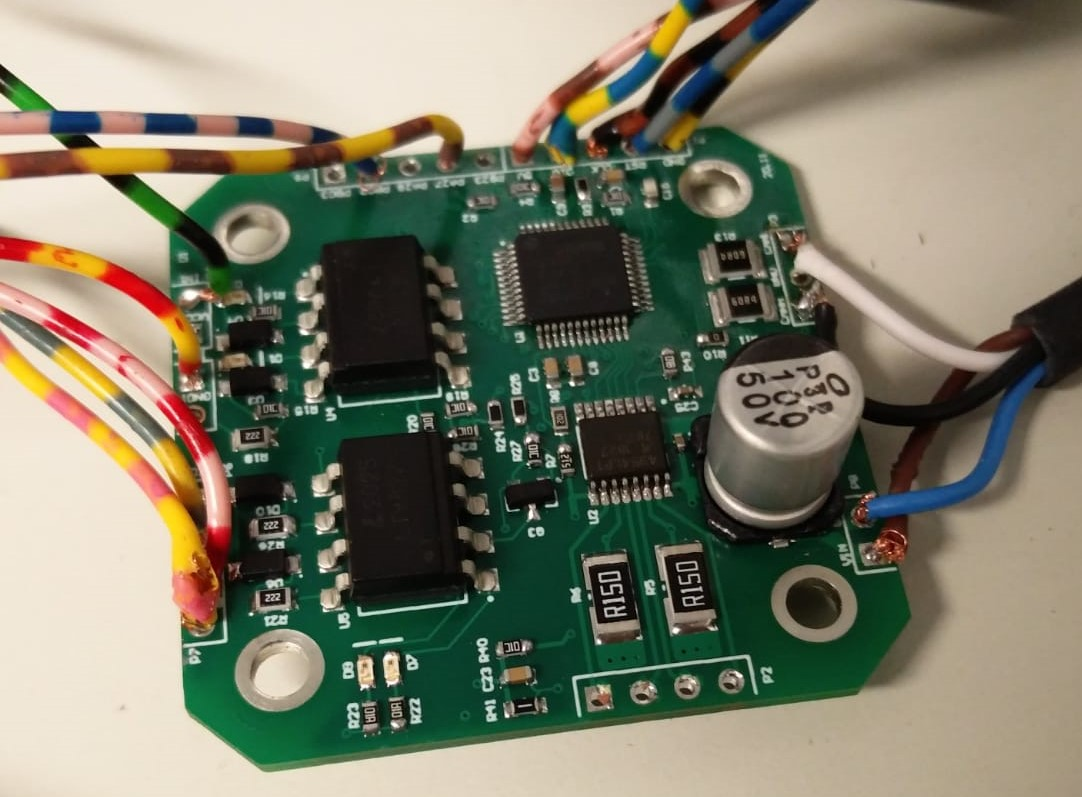
\includegraphics[scale=.3]{./Figures/SN17_5.jpeg}
	\caption{Plaqueta SN-17}
	\label{fig:SN17}
\end{figure}

Además de generar las funcionalidades mencionadas, el sistema SN-17 tiene señales discretas industriales que le permiten comunicarse a través de ese medio con controladores industriales (\textit{Programmable Logic Controllers} o PLCs) o pueden controlar un pequeño proceso por su cuenta.

Actualmente, se está trabajando en implementar estos sistemas en la planta de la empresa Cambre ICyFSA, donde se están construyendo distintos dispositivos para aplicaciones industriales con estos motores. En la Figura \ref{fig:aplicacionSN17} se puede observar un dibujo CAD de un actuador lineal con un sistema SN-17 implementado. Este funciona como un prensador en un proceso industrial.

\begin{figure}[htbp]
	\centering
	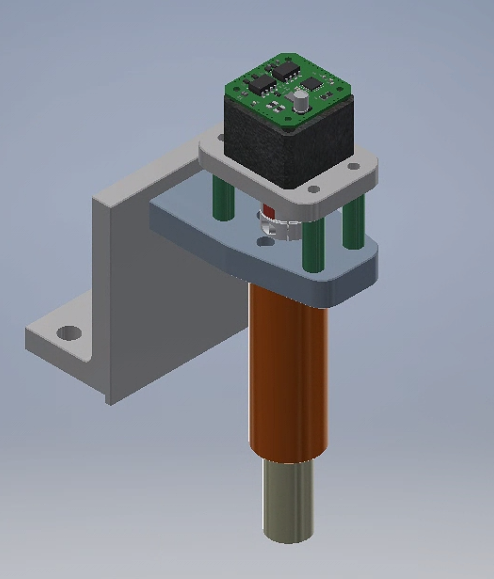
\includegraphics[scale=.6]{./Figures/Prensador-N17.PNG}
	\caption{Actuador lineal con SN-17}
	\label{fig:aplicacionSN17}
\end{figure}

%----------------------------------------------------------------------------------------

\section{Motivación}

En la actualidad, el ámbito de actuadores industriales está principalmente dominado por aquellos de carácter neumático. Sin embargo, en los últimos años, el uso de actuadores eléctricos ha empezado a ser más significativo debido a las mayores aptitudes de control que estos poseen. Estos suelen emplear un servomotor en su interior, y junto con un mecanismo generan el movimiento deseado con una precisión superior. Aún así, este tipo de actuadores tienen un problema en su elevado costo, que termina limitando su uso. En este contexto, la organización A3 Engineering desarrolló el sistema SN-17 en un intento de disminuir los costos de los servomotores de aplicaciones pequeñas y, en un futuro, de los actuadores eléctricos.

El sistema SN-17 cuenta con un problema a la hora de su utilización: la programación de los motores es compleja y se requiere de altos conocimientos técnicos para realizar modificaciones. Esto se debe a que, para cambiar las instrucciones del programa, es necesario modificar el firmware del sistema. Cuando se implementó inicialmente en planta, el sistema funcionó de forma exitosa, pero poco flexible. 

Con esta situación, se planteó la necesidad de que un técnico de planta sin mucho entrenamiento pudiera cambiar la programación y parámetros de funcionamiento de los motores. También, se consideró que sería conveniente, para maquinarias con varios motores conectados, poder hacer que todos estén dentro de una misma red, permitiendo así controles sobre conjuntos de motores.


%----------------------------------------------------------------------------------------

\section{Estado del arte}

Actualmente existe una gran oferta de servomotores y motores paso a paso. En general, lo que en el ámbito industrial se refiere a servomotores\citep{Industrial_Automation_Hands_On} son motores del tipo DC \textit{brushless} o AC de inducción (monofásicos y trifásicos). Estos tienen un valor significativamente mayor que los \textit{steppers} y suelen requerir de \textit{drivers} externos y, en caso de motores AC, variadores de frecuencia, convirtiendolos en soluciones de alto costo. En los casos que se requiere alta potencia o muy alto rendimiento, estos son la mejor opción. Suelen requerir de técnicos muy capacitados para su programación y suelen ofrecer interfaces de usuario avanzadas.

Por otro lado, en lo referido a motores \textit{steppers}, la oferta también es variada. Estos pueden adquirirse a precios muy accesibles y en distintos tamaños con lazo abierto. Requieren el uso de un \textit{driver} externo para su operación, y su programación suele hacerse con programas de terceros. Dependiendo la aplicación, pueden requerir de conocimientos técnicos elevados. También existen variantes que agregan un encoder de posición angular, comúnmente llamados \textit{closedloop steppers}. Estos solventan uno de los mayores problemas de estos motores, relacionado con la pérdida de posición en caso de una perturbación, pero no permiten entregar torque constante. También requieren de \textit{drivers} externos y, según el fabricante, las interfaces de programación pueden ser complejas.

Finalmente, existen placas de control que, además de funcionar como un \textit{closed loop stepper}, tienen un \textit{driver} incorporado que permite alimentar las bobinas de una forma diferente, logrando entregar torques constantes. El problema principal de estas soluciones es que suelen tener características de \textit{hobbista} y no son aplicables en ámbitos industriales y, además, suelen requerir mucho conocimiento técnico para su programación. En la Figura \ref{fig:mechaduino} se puede ver un ejemplo de una de estas placas llamado \textit{Mechaduino} \citep{web_mechaduino}.

\begin{figure}[htbp]
	\centering
	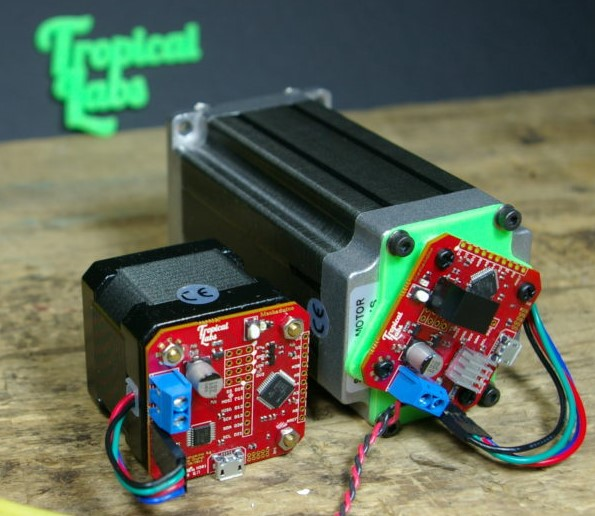
\includegraphics[scale=.6]{./Figures/mechaduino.jpg}
	\caption{Proyecto Mechaduino\protect\footnotemark}
	\label{fig:mechaduino}
\end{figure}

\footnotetext{\url{https://tropical-labs.com/mechaduino/}} %Link a imagen de mechaduino

En la Tabla \ref{tab:servos} se resume la información explicada en esta sección.


\begin{table}[h]
	\centering
	\caption[Estado del arte]{Resumen de características de servomotores}
	\begin{tabular}{c c c c c c}    
		\toprule
		\textbf{Motor} 	 & \textbf{Control}  & \textbf{Driver} & \textbf{Programación} & \textbf{Industrial} & \textbf{Precio (USD)} \\
		\midrule
		Servomotor & Lazo cerrado & Externo & Complejo & Sí	& > \$ 1.500 \\		
		\textit{Stepper open loop} & Lazo abierto & Externo & Intermedio & Sí	& \$ 300\\
		\textit{Stepper closed loop} & L. Cerrado s/torque	& Externo & Intermedio & Sí	& \$ 400\\
		\textit{Mechaduino} & Lazo cerrado	& Interno & Complejo & No	& \$ 200 \\
		SN-17 + interfaz	& Lazo cerrado	& Interno & Simple & Sí		& \$ 300 \\
		\bottomrule
		\hline
	\end{tabular}
	\label{tab:servos}
\end{table}
%----------------------------------------------------------------------------------------

\section{Objetivos y alcance}

El objetivo de este trabajo es proporcionar una interfaz de usuario para el sistema SN-17 que permita que un operario, con poco entrenamiento, pueda modificar los programas de los disntintos motores conectados a través de una red CAN con el sistema desarrollado. A su vez, debe poder emplearse para monitorear el estado los motores conectados cuando están operativos. Por lo tanto, el proyecto incluye:

\begin{itemize}
	\item Una interfaz de usuario que permita configurar y supervisar los servomotores conectados.
	\item La construcción e implementación de la estructura de mensajes CAN.
	\item La configuración de la red CAN.
	\item El desarrollo y fabricación de una plaqueta con el sistema embebido.
	\item El desarrollo del firmware para este sistema y la adaptación del firmware del sistema SN-17.
\end{itemize}


